\section{Multiplieur modulaire quantique de Beauregard}
Stéphane Beauregard propose aussi une manière de réaliser un multiplieur modulaire quantique qui utilise beaucoup moins de qubits que l'approche de Pavlidis \cite{beauregard2003circuitshorsalgorithmusing}. Cela rend la méthode intéressante, car les ressources étant moindres, on va pouvoir exécuter le circuit qui en découle et faire des tests. On présente quelques sous-routines qui, lorsque combinées, permettront de réaliser le multiplieur modulaire.

\subsection{C$\Phi$ADD$_a$ et CC$\Phi$ADD$_a$}
Tout d'abord, il nous faut des versions contrôlées de $\Phi$ADD$_a$. Construire ces portes n'est pas compliqué, car il suffit d'ajouter un ou deux qubits qui contrôlent l'application de chaque $A_{j+1}$ de la figure 6.

\begin{figure}[H]
    \begin{center}
        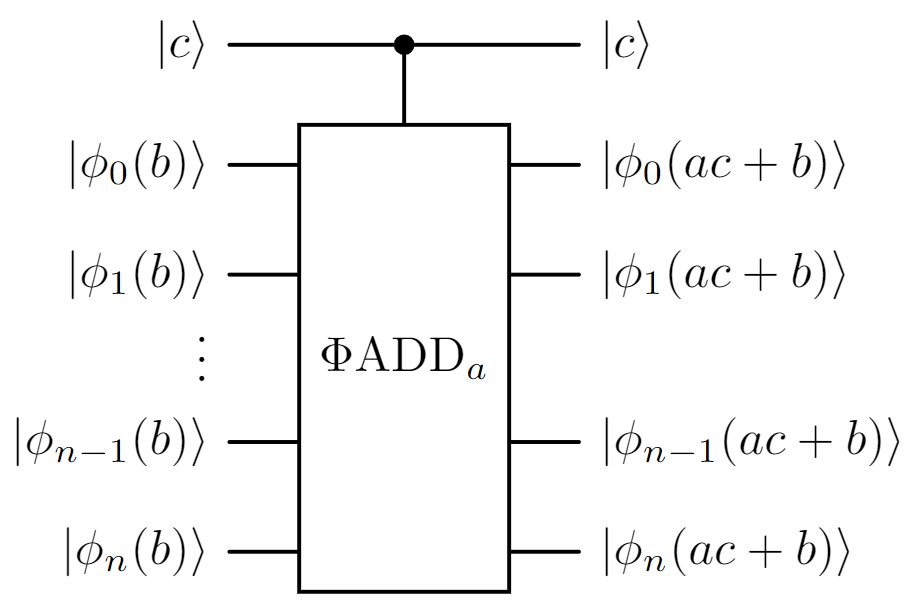
\includegraphics[scale=0.31]{images/cphiadd.png} 
        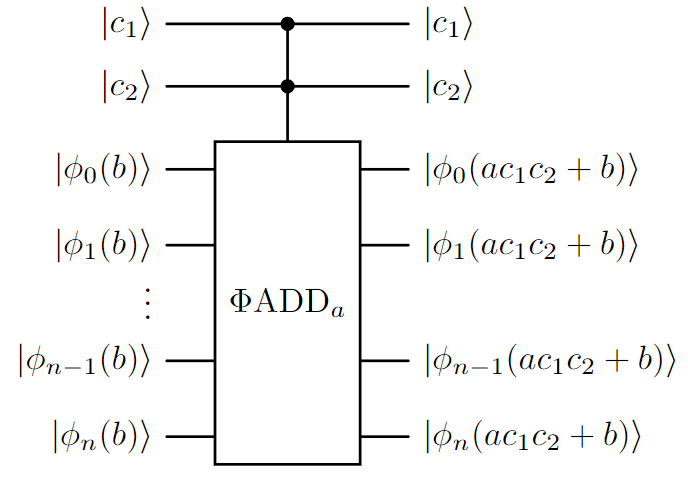
\includegraphics[scale=0.46]{images/ccphiadd.png}
        \caption{La porte C$\Phi$ADD$_a$ (à gauche) et la porte  CC$\Phi$ADD$_a$ (à droite)}   
    \end{center}
\end{figure}

\subsection{Additionneur modulaire CC$\Phi$ADD$_a$MOD$_N$}
L'additionneur modulaire prend des entiers positifs $a, b$ et $N$ sur $n$ bits où $a,b < N$. On utilisera ces quantités sur $n+1$ bits encore une fois pour gérer le débordement. L'additionneur modulaire permet de calculer $(a+b)\text{ mod } N$, c'est-à-dire de calculer $a+b$ et d'enlever $N$ si $a+b \geq N$.

 Comme préparation, on stocke $b$ dans un registre quantique à $n+1$ qubits et on lui applique la QFT pour avoir $\ket*{\phi(b)}$. En plus d'un qubit ancillaire $\ket*{0}$, il y a aussi deux qubits de contrôle $\ket*{c_1} $ et $\ket*{c_2}$. On s'attend donc à ce que  CC$\Phi$ADD$_a$MOD$_N (\ket*{c_1} \ket*{c_2} \ket*{\phi(b)} \ket*{0}) = \ket*{c_1}\ket*{c_2} \ket*{\phi((a\cdot c_1 c_2+b) \text{ mod } N)} \ket*{0}$. On présente d'abord le circuit correspondant à  CC$\Phi$ADD$_a$MOD$_N$, puis les détails mathématiques.

\begin{figure}[H]
    \centering
    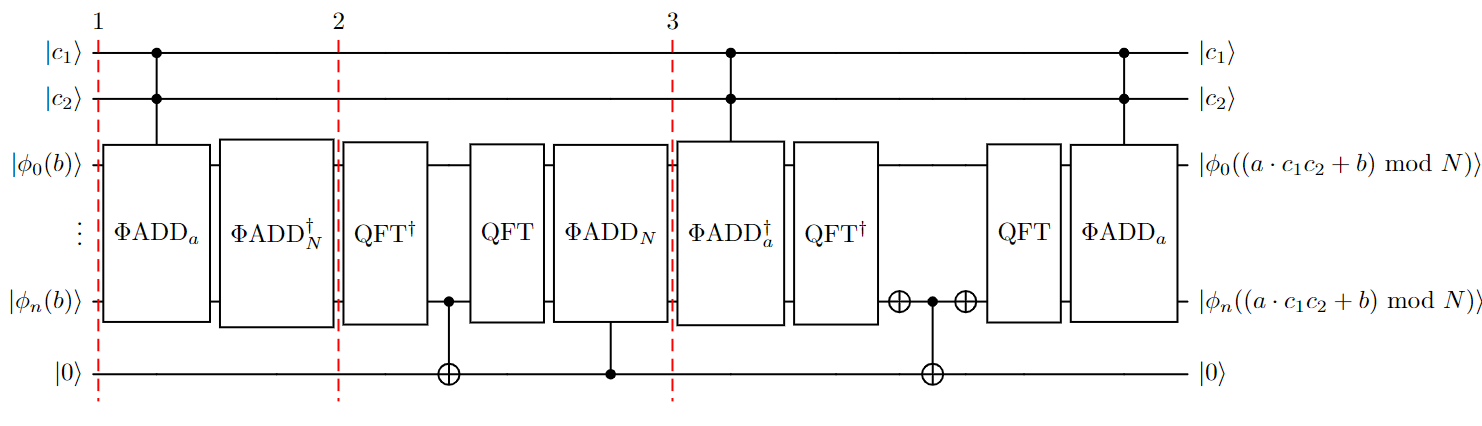
\includegraphics[scale=0.55]{images/add_mod.png}
    \caption{Circuit pour CC$\Phi$ADD$_a$MOD$_N$}
\end{figure}

\subsubsection*{Partie 1}
On commence par appliquer CC$\Phi$ADD$_a$ sur $\ket*{\phi(b)}$ pour avoir $\ket*{\phi(a \cdot c_1c_2 + b)}$. Puis, on utilise $\Phi$ADD$_N^\dag$ pour avoir $\ket*{\phi(a \cdot c_1c_2 + b - N)}$. On distingue alors deux cas. D'abord, il se peut que $a \cdot c_1c_2 + b - N < 0$, ce qui veut dire qu'on n'avait pas à soustraitre $N$ pour calculer le modulo. Puis, il est possible que $a \cdot c_1c_2 + b - N \geq 0$, ce qui indique que la soustraction par $N$ était nécessaire pour faire le modulo. 

\subsubsection*{Partie 2}
Pour savoir si on doit ou non rajouter $N$ pour calculer correctement le modulo, il faut avoir accès à la valeur du qubit de poids fort de $\ket*{a \cdot c_1c_2 + b - N}$. Effectivement, selon la section 6.3, il vaut 0 si $a \cdot c_1c_2 + b - N \geq 0$ et 1 sinon. Pour y arriver, il faut appliquer la QFT inverse sur $\ket*{\phi(a \cdot c_1c_2 + b - N)}$, puis copier la valeur du qubit de poids fort dans le qubit ancillaire grâce à une porte CNOT. On réapplique ensuite la QFT pour revenir à $\ket*{\phi(a \cdot c_1c_2 + b - N)}$. Si le qubit ancillaire vaut $\ket*{0}$, le modulo a été calculé correctement et il ne faut pas additionner $N$. Cependant, si le qubit ancillaire est dans l'état $\ket*{1}$, il faut rajouter $N$. Donc, il suffit d'utiliser C$\Phi$ADD$_N$ sur $\ket*{\phi(a \cdot c_1c_2 + b - N)}$ qu'on contrôle par le qubit ancillaire pour obtenir $\ket*{\phi((a \cdot c_1c_2 + b) \text{ mod } N)}$. 

\subsubsection*{Partie 3}
Il faut maintenant réinitialiser le qubit ancillaire à $\ket*{0}$. Pour ce faire, on se base sur l'identité suivante :

\begin{equation*}
    (a \cdot c_1 c_2 +b) \text{ mod } N \geq a \cdot c_1c_2 \iff a\cdot c_1c_2+b-N < 0
\end{equation*}
 
On sait donc que si $(a \cdot c_1 c_2 +b) \text{ mod } N \geq a \cdot c_1c_2$, alors le qubit ancillaire est à $\ket*{1}$. Sinon, il est à $\ket*{0}$. On utilise CC$\Phi$ADD$_a^\dag$ pour soustraire $a \cdot c_1c_2$ de $\ket*{\phi((a \cdot c_1c_2 + b) \text{ mod } N)}$, puis on applique la QFT inverse. Cette fois, selon l'identité, le qubit de poids fort vaut $\ket*{0}$ si $a\cdot c_1c_2+b-N < 0$ (donc le qubit ancillaire est forcément $\ket*{1}$) et $\ket*{1}$ sinon (donc le qubit ancillaire est forcément $\ket*{0}$). Pour faire la correction appropriée sur le qubit ancillaire, on inverse la valeur du qubit de poids fort qui contrôle ensuite une porte CNOT sur le qubit ancillaire. On vient alors de réinitialiser le qubit ancillaire et le reste du circuit ramène le qubit de poids fort à sa bonne valeur avant de rajouter $a \cdot c_1c_2$. Pour résumer, on a calculé le modulo et le qubit ancillaire est de retour à $\ket*{0}$.

Finalement, l'inverse de l'additionneur modulaire produit $\ket*{\phi(b - a \cdot c_1c_2)}$ si $b \geq a$ et $\ket*{\phi(b - a \cdot c_1c_2 + N)}$ sinon, ce qui est équivalent pour les deux cas à $\ket*{\phi((b- a \cdot c_1c_2) \text{ mod } N)}$. 

\subsection{Multipieur modulaire C$\Phi$MULT$_a$MOD$_N$}
Pour des entiers positifs  $a, b, x$ et  $N$ sur $n$ bits, le mutiplieur modulaire calcule $(b + ax) \text{ mod } N$. Puisque $x = \sum_{j=0}^{n-1}x_j 2^j$, il va de soi que $(b + ax) \text{ mod } N = (b + ax_02^0 + ... + ax_{n-1}2^{n-1}) \text{ mod } N$. En utilisant les identités de la section 1, on a 

\begin{equation*}
    (b + ax_02^0 + ... + ax_{n-1}2^{n-1}) \text{ mod } N = [(b + ax_02^0 + ... + ax_{n-2}2^{n-2})\text{ mod } N + (ax_{n-1}2^{n-1}) \text{ mod } N] \text{ mod } N 
\end{equation*}
\begin{equation*}
    = [((b + ax_02^0 + ... + ax_{n-3}2^{n-3}) \text{ mod } N + (ax_{n-2}2^{n-2}) \text{ mod } N) \text{ mod } N + (ax_{n-1}2^{n-1})\text{ mod }N]\text{ mod }N = ...
\end{equation*}
\begin{equation*}
    = [... ((b) \text{ mod } N + (ax_02^0)\text{ mod } N)\text{ mod } N + ... + (ax_{n-1}2^{n-1})\text{ mod } N]\text{ mod } N
\end{equation*}
\begin{equation*}
    = [... {\underbrace{(b + (ax_02^0)\text{ mod } N)\text{ mod } N}_\text{CC$\Phi$ADD$_{a2^0 \text{ mod } N}$MOD$_N$} + ... + (ax_{n-1}2^{n-1})\text{ mod } N]\text{ mod } N}
\end{equation*}

On voit alors que le multiplieur modulaire peut être réalisé en appliquant successivement CC$\Phi$ADD$_{a2^j \text{mod} N}$MOD$_N$ pour $j$ allant de 0 à $n-1$. Pour ce faire, on initialise un registre de $n$ qubits contenant $\ket*{x}$ et un qubit de contrôle $\ket*{c}$ s'ajoute aussi pour autoriser ou non l'opération. De nouveau, on prépare un second registre de $n+1$ qubits avec $\ket*{\phi(b)}$. Il y a aussi un qubit ancillaire nécessaire pour utiliser CC$\Phi$ADD$_a$MOD$_N$ qui est implicitement présent à la figure 10. Au total, il nous faut $2n+3$ qubits pour réaliser le multiplieur modulaire. L'opération désirée correspond donc à 

\begin{equation}
    \text{C}\Phi\text{MULT}_a\text{MOD}_N (a, N, \ket*{c}, \ket*{x}, \ket*{\phi(b)}) = \ket*{c} \ket*{x} \ket*{\phi((b + ax\cdot c) \text{ mod } N)}
\end{equation}

Il faut noter qu'il est nécessaire de calculer classiquement $2^j a \text{ mod } N$ avant de le donner en argument à chaque porte. De cette manière, toutes les valeurs vont tenir sur $n+1$ qubits et on diminue le nombre de qubits qu'il aurait fallu autrement pour faire le calcul. Le calcul classique du modulo se fait en temps polynomial. Pour terminer, C$\Phi$MULT$_a$MOD$_N^\dag$ permet de produire $\ket*{\phi((b - ax \cdot c)\text{ mod } N)}$.

\begin{figure}[H]
    \centering
    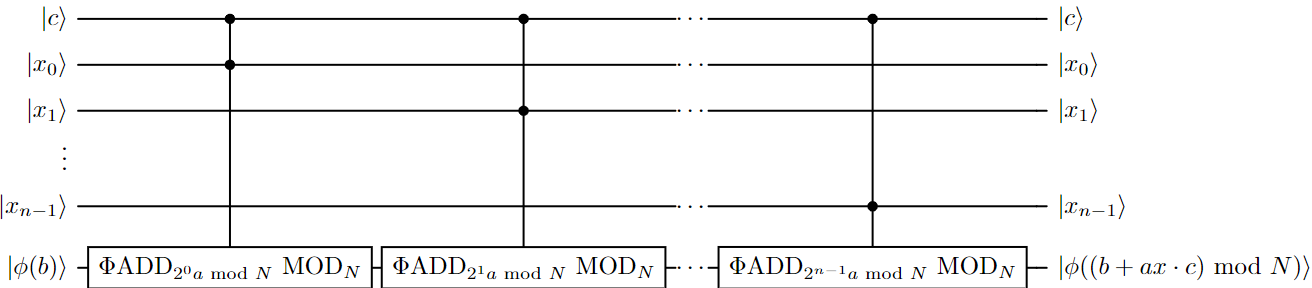
\includegraphics[scale=0.63]{images/phimultmod.png}
    \caption{Circuit pour le multiplieur modulaire C$\Phi$MULT$_a$MOD$_N$}
\end{figure}

\subsection{$CU_a$}
On a maintenant tous les blocs nécessaires pour faire la porte $CU_a$. D'abord, l'initialisation des registres est la même que pour la section précédente, sauf qu'on pose $b=0$. De plus, on rajoute comme condition que pgcd($a, N$) = 1. Puis, on applique C$\Phi$MULT$_a$MOD$_N$ afin d'avoir $\ket*{x}$ sur le premier registre et $\ket*{ax \text{ mod } N}$ sur le deuxième registre (après la porte QFT$^\dag$). Ensuite, une porte SWAP contrôlée par $\ket*{c}$ échange tout le premier registre avec les $n$ premiers qubits du deuxième registre, ce qui amène  $\ket*{ax \text{ mod } N}$ sur le premier registre et $\ket*{\phi(x)}$ sur le second (après la porte QFT). Finalement, une porte C$\Phi$MULT$_{a^{-1}}$MOD$_N^\dag$ permet de réinitialiser le deuxième registre à $\ket*{\phi(0)}$ tout en gardant $\ket*{ax \text{ mod } N}$ dans le premier registre. On rappelle que $a^{-1}$ est l'inverse multiplicatif modulo $N$ de $a$ qui existe grâce au fait que pgcd($a, N$) = 1. Donc, C$\Phi$MULT$_{a^{-1}}$MOD$_N^\dag$ change $\ket*{\phi(x)}$ pour l'état $\ket*{\phi((x - a^{-1}(ax \text{ mod } N)) \text{ mod } N)}$ sur le second registre qui équivaut, en utilisant les identités de la section 1, à $\ket*{(x - a^{-1}a x) \text{ mod } N}$. Comme on sait que $a^{-1}a \equiv 1 \text{ mod } N$, l'état final correspond en fait à $\ket*{\phi(x - 1  \cdot x)\text{ mod } N} = \ket*{\phi(0)}$. Au final, on retrouve bien la porte $CU_a$.

\begin{figure}[H]
    \centering
    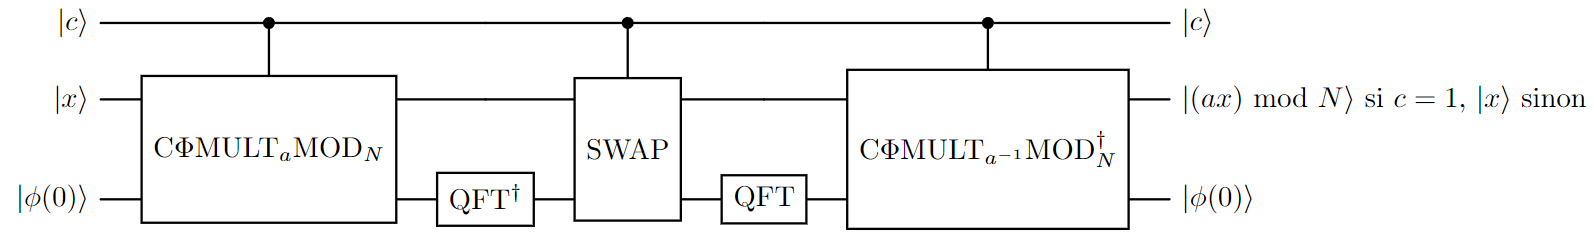
\includegraphics[scale=0.4]{images/CU_x.png}
    \caption{Circuit pour $CU_a$}
\end{figure}

Si on se ramène à la section sur le problème de la recherche d'ordre, on voudrait appliquer $CU_a^{2^k}$. En fait, $U_a^{2^k} \ket*{x} = \ket*{a^{2^k} \text{ mod }N } = U_{a^{2^k}} \ket*{x}$ où on peut calculer classiquement $a^{2^k}$ en temps polynomial. Dès lors, on peut résoudre la recherche d'ordre à l'aide de la QPE. Au final, la recherche d'ordre nécessite $2n + 2 + m$ qubits où $m$ est le nombre de qubits de précision de la QPE. Avec le \textit{one qubit trick}, le nombre de qubits diminue à $2n + 3$. Globalement, la recherche d'ordre avec la méthode de Beauregard a une complexité polynomiale \cite{beauregard2003circuitshorsalgorithmusing}.